\documentclass{article}
\usepackage[utf8]{inputenc}
\usepackage{geometry}
\usepackage{graphicx}
\usepackage{amsmath}
\usepackage{amsfonts}
\usepackage{amsthm}
\usepackage{amssymb}
% \usepackage[most]{tcolorbox}
\usepackage{array}
\usepackage{latexsym}
\usepackage{alltt}
\usepackage{hyperref}
\usepackage{color, colortbl}
\usepackage{float}
\usepackage{pdfpages}
\usepackage{algpseudocode}
\usepackage{multicol}
\usepackage{multirow}
\usepackage{caption}
\usepackage{xparse}
\usepackage{setspace}
\usepackage{enumitem}
\usepackage{pdflscape}
% \usepackage{parskip}
\usepackage{blindtext}
\usepackage{forest}
\usepackage[newfloat]{minted}
\usepackage{booktabs}
\usepackage[most, minted]{tcolorbox}


\geometry
{
  a4paper,
  left=12mm,
  right=12mm,
  top=12mm,
  bottom=15mm,
}

% mybox
\newtcolorbox{mybox}[3][]
{
  colframe = #2!25,
  colback  = #2!10,
  coltitle = #2!20!black,  
  title    = {#3},
  #1,
}

\definecolor{ex}{rgb}{1.00,0.65,0.00}
\definecolor{bg}{rgb}{0.95,0.95,0.95}


\newtcblisting{myminted}{%
    listing engine=minted,
    minted language=matlab,
    listing only,
    breakable,
    enhanced,
    minted options = {
        linenos, 
        breaklines=true, 
        breakbefore=., 
        fontsize=\footnotesize, 
        numbersep=2mm
    },
    overlay={%
        \begin{tcbclipinterior}
            \fill[gray!25] (frame.south west) rectangle ([xshift=4mm]frame.north west);
        \end{tcbclipinterior}
    }   
}

\SetupFloatingEnvironment{listing}{name=Code}

% New environments that use mybox
\newcounter{example}[section]
\newenvironment{example}[1]{\begin{mybox}[breakable]{ex}{\refstepcounter{example}\textbf{Example \thesection.\theexample #1}}}{\end{mybox}}

\newcounter{definition}[section]
\newenvironment{definition}[1]{\refstepcounter{definition}\begin{mybox}[breakable]{blue}{\textbf{Definition \thesection.\thedefinition #1}}}{\end{mybox}}

\newcounter{theorem}[section]
\newenvironment{theorem}[1]{\begin{mybox}{red}{\refstepcounter{theorem}\textbf{Theorem \thesection.\thetheorem #1}}}{\end{mybox}}

\newenvironment{formula}[1]{\begin{mybox}{cyan}{\textbf{#1}}}{\end{mybox}}

% Changing maketitle
\makeatletter         
\renewcommand\maketitle{
{\raggedright % Note the extra {
\begin{center}
{\Large \bfseries \@title}\\[2ex] 
{\large \@author \ - \@date}\\[2ex]
\end{center}}} % Note the extra }
\makeatother

% \onehalfspacing % adjust spacing
\setlength{\parskip}{0.5\baselineskip}

% macros
\newcommand{\prob}[1]{\textbf{\textit{P}}\left\{#1\right\}}
\newcommand{\expc}[1]{\mathbf{E}\left(#1\right)}
\newcommand{\expcs}[1]{\mathbf{E}^2\left(#1\right)}
\newcommand{\var}[1]{\text{Var}\left( #1 \right)}
\newcommand{\ra}{\rightarrow}
\newcommand{\la}{\leftarrow}
\newcommand{\tar}{\vartriangleright}
\newcommand{\Ra}{\Rightarrow}
\newcommand{\blank}{\sqcup}
\newcommand{\R}[2]{\tikz [remember picture,overlay] \node (#1) {#2};}

\def\circtxt#1{$\mathalpha \bigcirc \mkern-13mu \mathtt #1$}
\def\smiley{\textcircled{\scriptsize $\mkern3mu\ddot{\ } \mkern-15mu \smallsmile$}}

\NewDocumentCommand{\dsum}{%
    e{^_}
}{%
  {% 
    \displaystyle\sum
    \IfValueT{#1}{^{#1}}
    \IfValueT{#2}{_{#2}}
  }
}%

% maketitle variables
\title{Title}
\author{Burak Metehan Tunçel}
\date{\today}

\begin{document}

\section*{Student Information}

\noindent \textbf{Full Name:} Burak Metehan Tunçel

\noindent \textbf{Id Number:} 2468726

\section*{Answer 1}

\subsection*{a)}

\noindent \textit{They are \textbf{not independent}}. Independence formula for continuous variables is
\begin{equation*}
    f_{(X, Y)} (x, y) = f_X(x) f_Y(y)
\end{equation*}
So, we need to find equations for $f_X(x)$ and $f_Y(y)$.

\subsubsection*{Finding $f_X(x)$}

\begin{equation*}
    f_X(x) = \int_{-\infty}^{\infty} f_{(X, Y)} (x, y) dy
\end{equation*}

\noindent We can rewrite the function $f_{(X, Y)}(x, y)$ as follows,
\begin{equation*}
    f_{(X, Y)}(x, y) = \begin{cases}
        \dfrac{1}{\pi} &\textnormal{if $-\sqrt{1-x^2} \leq y \leq \sqrt{1-x^2}$}\\
        0 &\textnormal{otherwise}
    \end{cases}
\end{equation*}
One can say that for otherwise part, the integral is 0. For other part,
\begin{align*}
    f_X(x) &= \int_{-\sqrt{1-x^2}}^{\sqrt{1-x^2}} f_{(X, Y)}(x, y) dy\\
         &= \int_{-\sqrt{1-x^2}}^{\sqrt{1-x^2}} \frac{1}{\pi} dy\\
         &= \frac{2\sqrt{1-x^2}}{\pi} &-1 \leq x \leq 1
\end{align*}

\subsubsection*{Finding $f_Y(y)$}

\noindent Similarly, we can rewrite the function $f_{(X, Y)}(x, y)$ as follows,
\begin{equation*}
    f_{(X, Y)}(x, y) = \begin{cases}
        \dfrac{1}{\pi} &\textnormal{if $-\sqrt{1-y^2} \leq x \leq \sqrt{1-y^2}$}\\
        0 &\textnormal{otherwise}
    \end{cases}
\end{equation*}
From here,
\begin{align*}
    f_Y(y) &= \int_{-\sqrt{1-y^2}}^{\sqrt{1-y^2}} f_{(X, Y)}(x, y) dx\\
         &= \int_{-\sqrt{1-y^2}}^{\sqrt{1-y^2}} \frac{1}{\pi} dx\\
         &= \frac{2\sqrt{1-y^2}}{\pi} &-1 \leq y \leq 1
\end{align*}

\noindent In the end, we have
\begin{align*}
    f_X(x) &= \begin{cases}
                \dfrac{2\sqrt{1-x^2}}{\pi} &-1 \leq x \leq 1\\
                0 &\textnormal{otherwise}
            \end{cases}\\
    f_Y(y) &= \begin{cases}
                \dfrac{2\sqrt{1-y^2}}{\pi} &-1 \leq y \leq 1\\
                0 &\textnormal{otherwise}
            \end{cases}
\end{align*}

\noindent So back to formula
\begin{equation*}
    \left[ f_{(X, Y)}(x, y) = \begin{cases}
        \dfrac{1}{\pi} &x^2 + y^2 \leq 1\\
        0 &\textnormal{otherwise}
    \end{cases} \right]\
    \
    \
    \neq \left[ f_X(x) f_Y(y) = \begin{cases}
        \dfrac{2\sqrt{1-x^2}}{\pi} \cdot \dfrac{2\sqrt{1-y^2}}{\pi} &-1 \leq x \leq 1, -1 \leq y \leq 1\\
        0 &\textnormal{otherwise}
    \end{cases} \right]
\end{equation*}

\noindent Also, we can show that they are dependent if we find at least 1 pair that violates the independecy equation. Let $x = y = \dfrac{\sqrt{3}}{2}$, then
\begin{equation*}
    f_{(X, Y)}\left(\dfrac{\sqrt{3}}{2}, \dfrac{\sqrt{3}}{2}\right) = \frac{1}{\pi} \neq \frac{1}{\pi^2} = f_X\left(\dfrac{\sqrt{3}}{2}\right) f_Y\left(\dfrac{\sqrt{3}}{2}\right)
\end{equation*}

\subsection*{b)}

From part a,
\begin{align*}
    f_X(x) &= \begin{cases}
                \dfrac{2\sqrt{1-x^2}}{\pi} &-1 \leq x \leq 1\\
                0 &\textnormal{otherwise}
            \end{cases}\\
    f_Y(y) &= \begin{cases}
                \dfrac{2\sqrt{1-y^2}}{\pi} &-1 \leq y \leq 1\\
                0 &\textnormal{otherwise}
            \end{cases}
\end{align*}

\subsection*{c)}

Since our pdf is piecewise, we need the calculate each piece one by one,
\begin{align*}
    \expc{X} = \mu &= \int_{-\infty}^{\infty} x f_X(x) dx\\
                        &= \int_{-\infty}^{-1} x f_X(x) dx + \int_{-1}^{1} x f_X(x) dx + \int_{1}^{\infty} x f_X(x) dx\\
                        &= \int_{-\infty}^{-1} x 0 dx + \int_{-1}^{1} x \dfrac{2\sqrt{1-x^2}}{\pi} dx + \int_{1}^{\infty} x 0 dx\\
                        &= \int_{-\infty}^{-1} 0 dx + \int_{-1}^{1} x \dfrac{2\sqrt{1-x^2}}{\pi} dx + \int_{1}^{\infty} 0 dx\\
                        &= 0 + \left[ -\frac{2}{\pi} \cdot \frac{1}{3} \left( 1 - x^2 \right)^{\frac{3}{2}} \right]\Biggl|_{-1}^{1} + 0\\
                        &= \left[ -\frac{2}{\pi} \cdot \frac{1}{3} \left( 1 - 1^2 \right)^{\frac{3}{2}} \right] - \left[ -\frac{2}{\pi} \cdot \frac{1}{3} \left( 1 - (-1)^2 \right)^{\frac{3}{2}} \right]\\
                        &= 0 - 0 = 0
\end{align*}

\subsection*{d)}

Since our pdf is piecewise, we need the calculate each piece one by one,
\begin{align*}
    \var{X} &= \expc{X - \mu^2}^2\\
            &= \int_{-\infty}^{\infty} \left( x - \mu \right)^2 f_X(x) dx\ \ \ \ \ (\mu = 0)\\
            &= \int_{-\infty}^{\infty} x^2 f_X(x) dx\\
            &= \int_{-\infty}^{-1} x^2 f_X(x) dx + \int_{-1}^{1} x^2 f_X(x) dx + \int_{1}^{\infty} x^2 f_X(x) dx\\
            &= 0 + \int_{-1}^{1} x^2 \dfrac{2\sqrt{1-x^2}}{\pi} dx + 0\\
            &= \left[ \frac{1}{16\pi} \left( 4 \arcsin(x) - \sin(4\arcsin(x)) \right) \right] \Biggl|_{-1}^{1}\\
            &= \left[ \frac{1}{16\pi} \left( 4 \arcsin(1) - \sin(4\arcsin(1)) \right) \right] - \left[ \frac{1}{16\pi} \left( 4 \arcsin(-1) - \sin(4\arcsin(-1)) \right) \right]\\
            &= \left( \frac{1}{8} \right) - \left( -\frac{1}{8} \right)\\
            &= \frac{2}{8} = \frac{1}{4}
\end{align*}


\newpage
\section*{Answer 2}

\subsection*{a)}

\noindent Since $T_A$ and $T_B$ are uniformly distributed
\begin{align*}
  f_{T_A}(t_A) &= \frac{1}{100 - 0} = \frac{1}{100}\\
  f_{T_B}(t_B) &= \frac{1}{100 - 0} = \frac{1}{100}
\end{align*}

Also, since $T_A$ and $T_B$ are indenpendent,
\begin{align*}
  f_{(T_A, T_B)}(t_A, t_B) = f_{T_A}(t_A) f_{T_B}(t_B) = \frac{1}{100} \cdot \frac{1}{100} = \frac{1}{10000} = 10^{-4}
\end{align*}

We found joinst density function. Now we can find joint cdf. Let $u = t_A$, $v = t_B$, then
\begin{align*}
  F_{(X, Y)} (x, y) &= \int_{0}^{y} \int_{0}^{x} f_{(X, Y)} (u, v) du dv\\
  &= \int_{0}^{y} \int_{0}^{x} 10^{-4} du dv\\
  &= \int_{0}^{y} x \cdot 10^{-4} dv\\
  &= xy \cdot 10^{-4}
\end{align*}

\subsection*{b)}

\begin{formula}{}
  In joint cumulative function of two random variables $X$ and $Y$, $F_{(X, Y)} (x, y) = F_X(x) F_Y(y)$ if $X$ and $Y$ are independent. Also, notice that it happened in this question.
  \begin{align*}
      F_{T_A}(t_a) &= \int_{0}^{t_a} f_{T_A}(u)du = t_a \cdot 10^{-2}\\
      F_{T_B}(t_b) &= \int_{0}^{t_b} f_{T_B}(u)du = t_B \cdot 10^{-2}\\
      F_{(T_A, T_B)} (t_A, t_B) &=  F_{T_A}(t_a) \cdot F_{T_B}(t_b) = t_a t_b \cdot 10^{-4}
  \end{align*}
  This fact will be used in the following part.
\end{formula}

We are asked the following probability
\begin{equation*}
  \prob{0 \leq T_A \leq 10,\ 90 \leq T_B \leq 100}
\end{equation*}

We can write it as follows,

\begin{align*}
  \prob{0 \leq T_A \leq 10,\ 90 \leq T_B \leq 100} = F_{(T_A, T_B)} (t_A, t_B) = F_{T_A} (t_a) \cdot F_{T_B} (t_b)
\end{align*}

\subsubsection*{Calculating $F_{T_A} (t_a)$}

\begin{equation*}
  F_{T_A} (t_a) = \int_{0}^{10} f_{T_A} (u) du = \int_{0}^{10} 10^{-2} du = 10^{-2} \cdot 10 = 10^{-1}
\end{equation*}

\subsubsection*{Calculating $F_{T_B} (t_b)$}

\begin{equation*}
  F_{T_B} (t_b) = \int_{90}^{100} f_{T_B} (u) du = \int_{90}^{100} 10^{-2} du = 10^{-2} \cdot 10 = 10^{-1}
\end{equation*}

Then,

\begin{equation*}
  F_{T_A} (t_a) \cdot F_{T_B} (t_b) = 10^{-1} \cdot 10^{-1} = 10^{-2}
\end{equation*}

So the answer is $\dfrac{1}{100}$

\subsection*{c)}

% What is the probability that subject A pushes the button at most 20 seconds after subject B?

% Since it is mentioned that ``at most 20 seconds'', we can think the subject B will push at most in 80 secs and subject A will push. In other words, since $T_A, T_B \in \left[ 0, 100 \right]$, $ 

% We are asked the following
% \begin{align*}
%   \prob{T_B \leq T_A \leq T_B + 20,\ 0 \leq T_B \leq 100}
% \end{align*}

% So,

% \begin{align*}
%   \prob{T_B \leq T_A \leq T_B + 20,\ 0 \leq T_B \leq 100} &= \int_{x}^{y} \int_{0}^{100} f_{(X, Y)} (u, v) du dv\\
%   &= \int_{}^{} \int_{0}^{100} 10^{-2} du dv\\
%   &= \int_{}^{} dv
% \end{align*}

%%%%%%%%%%%%%%%%%%%%%%%%%%%%%%%%%%%

If we think like the way mentioned in the hint. We are asked the ratio of the purple area to all area $\left[ 100 \times 100 \right]$ calculate the probability of the area of the Figure 1. The area is the following
\begin{equation*}
  \prob{(T_A - T_B \leq 20) \cap (T_B \leq T_A)}
\end{equation*}

\begin{figure}[ht!]
  \centering
  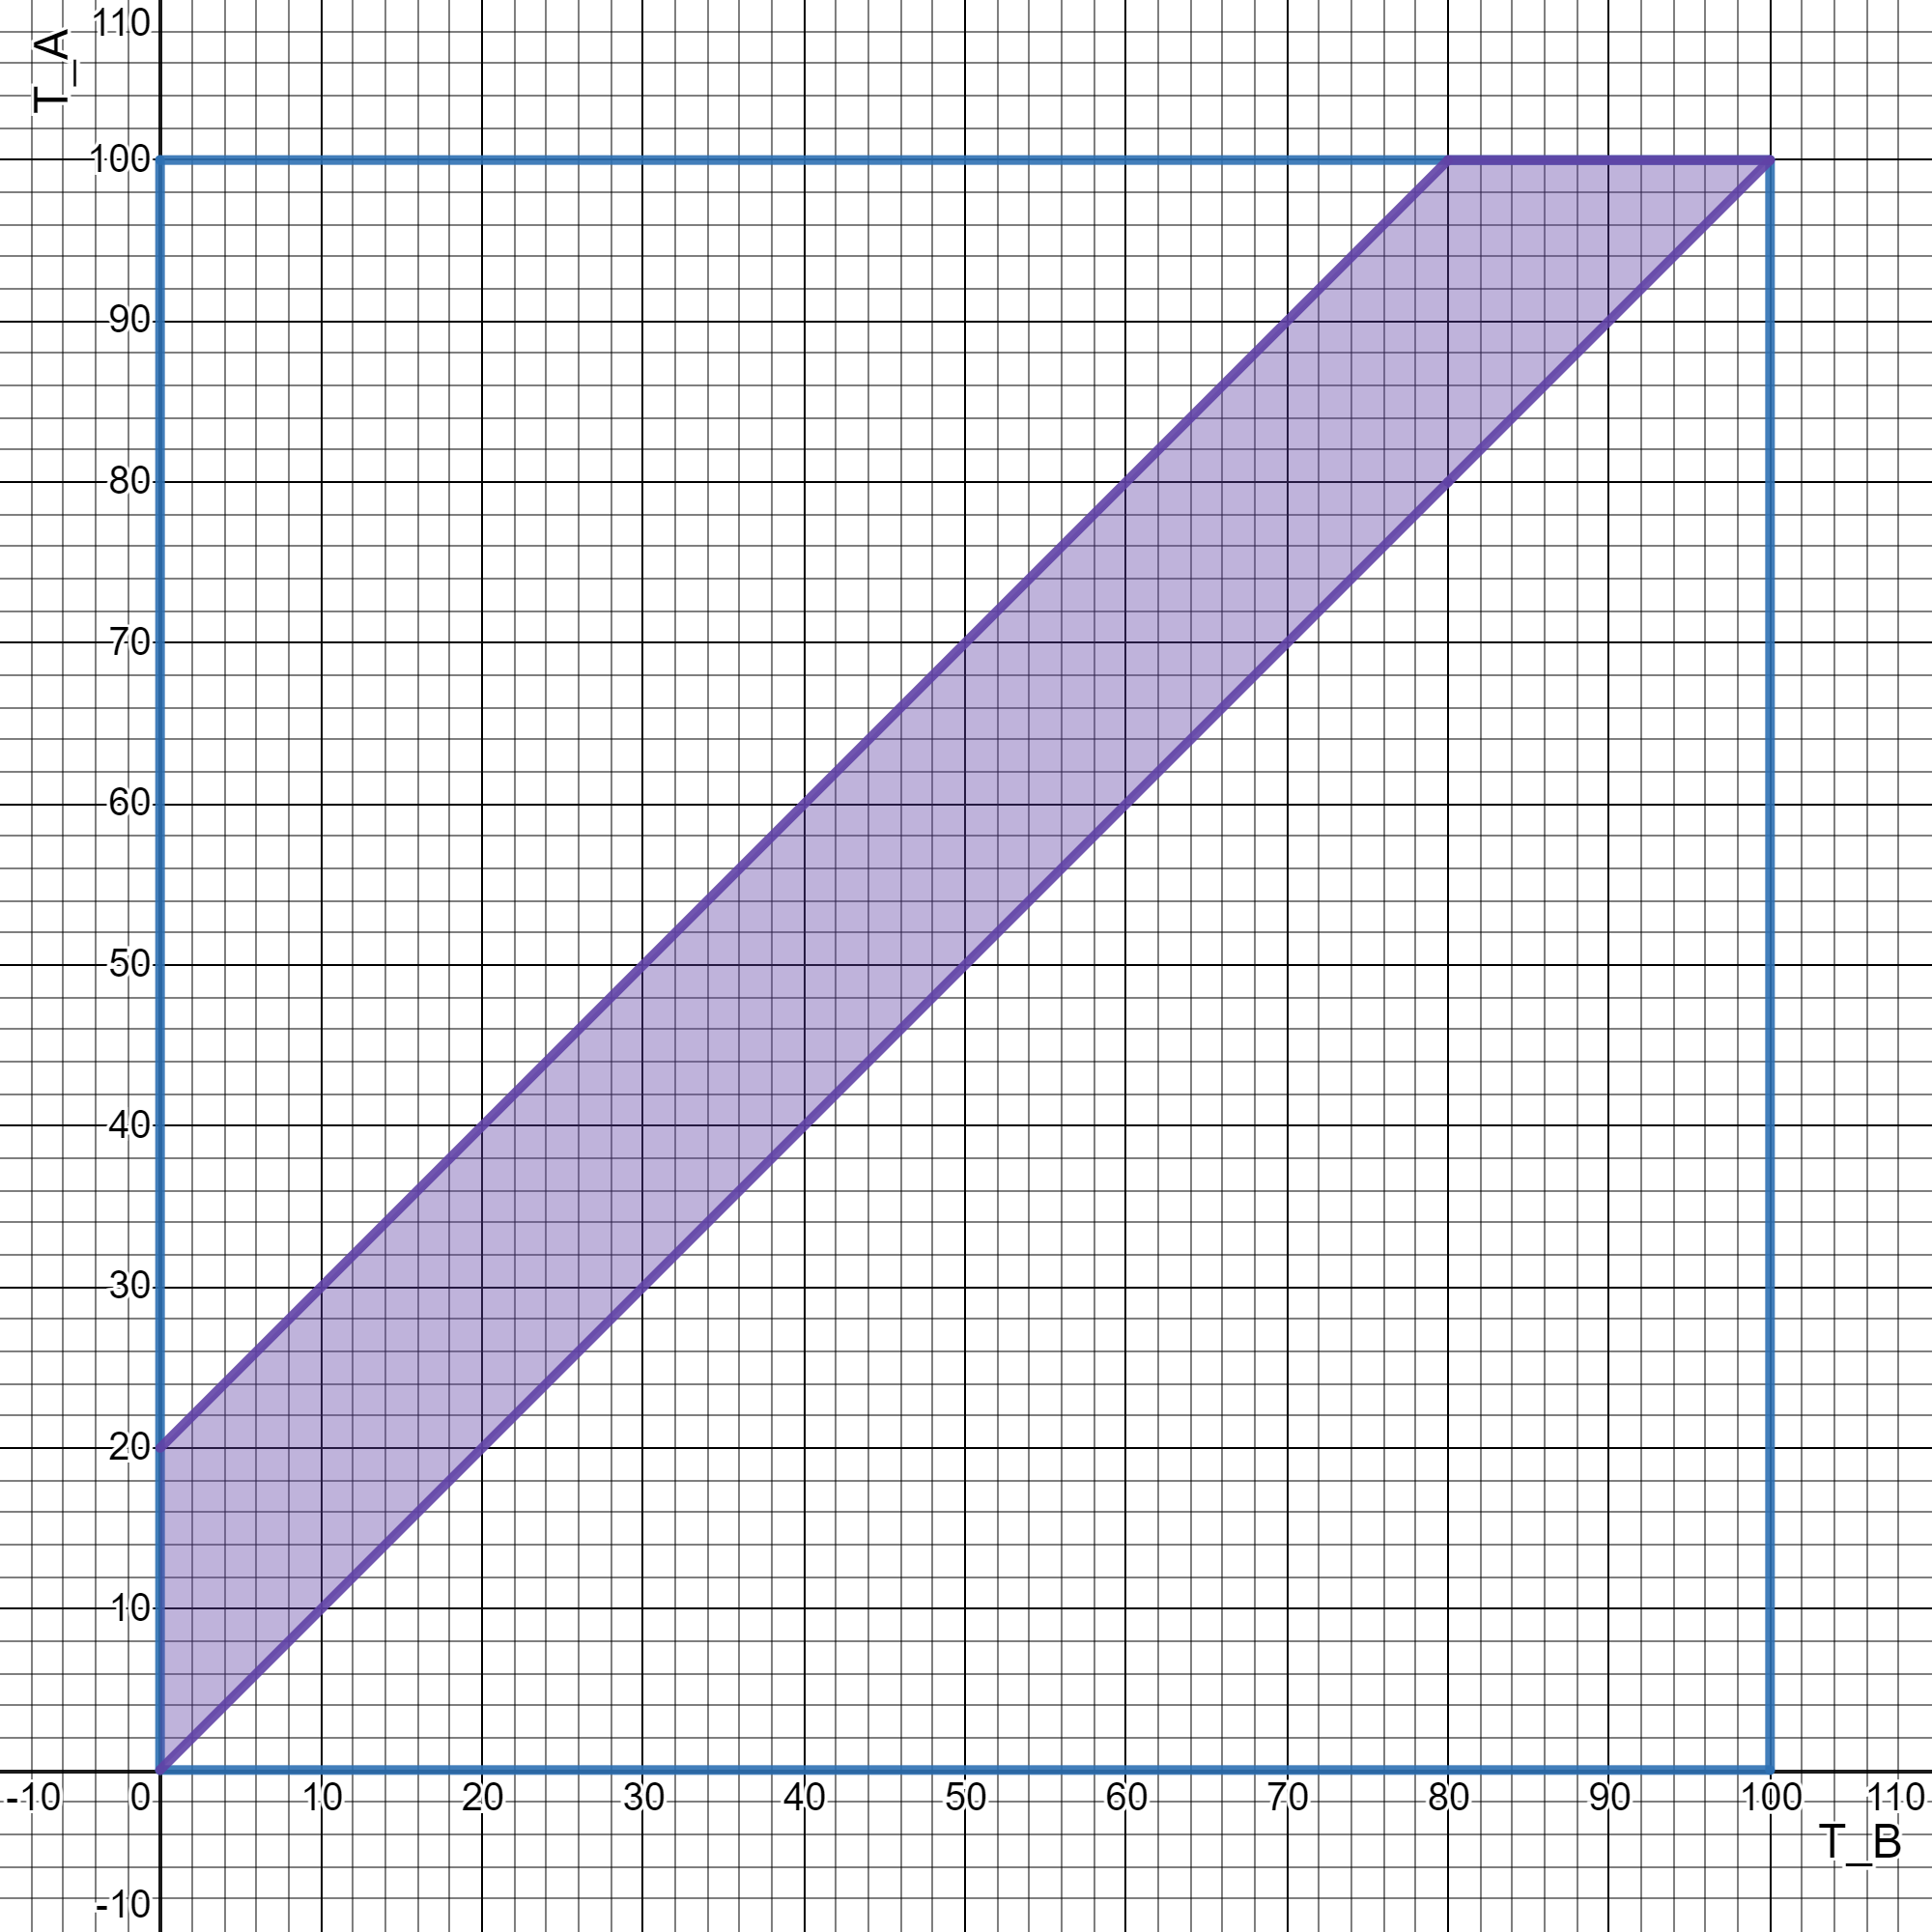
\includegraphics[width=.4\textwidth]{img/q2-c.png}
  \caption{}
\end{figure}

\begin{multicols}{2}
\begin{itemize}
  \item $\textnormal{The area of purple part} = 1800$
  \item $\textnormal{The area of the whole part} = 10^4$
\end{itemize}
\end{multicols}

So, the ratio of the purple area to whole area is the answer and it is $\dfrac{18}{100} = 0.18$.

\newpage
\subsection*{d)}

Again, if we think like the way mentioned in the hint. We are asked the ratio of the purple area to all area $\left[ 100 \times 100 \right]$ calculate the probability of the area of the Figure 2. The area is the following
\begin{equation*}
  \prob{(|T_A - T_B| \leq 30)}
\end{equation*}

\begin{figure}[ht!]
  \centering
  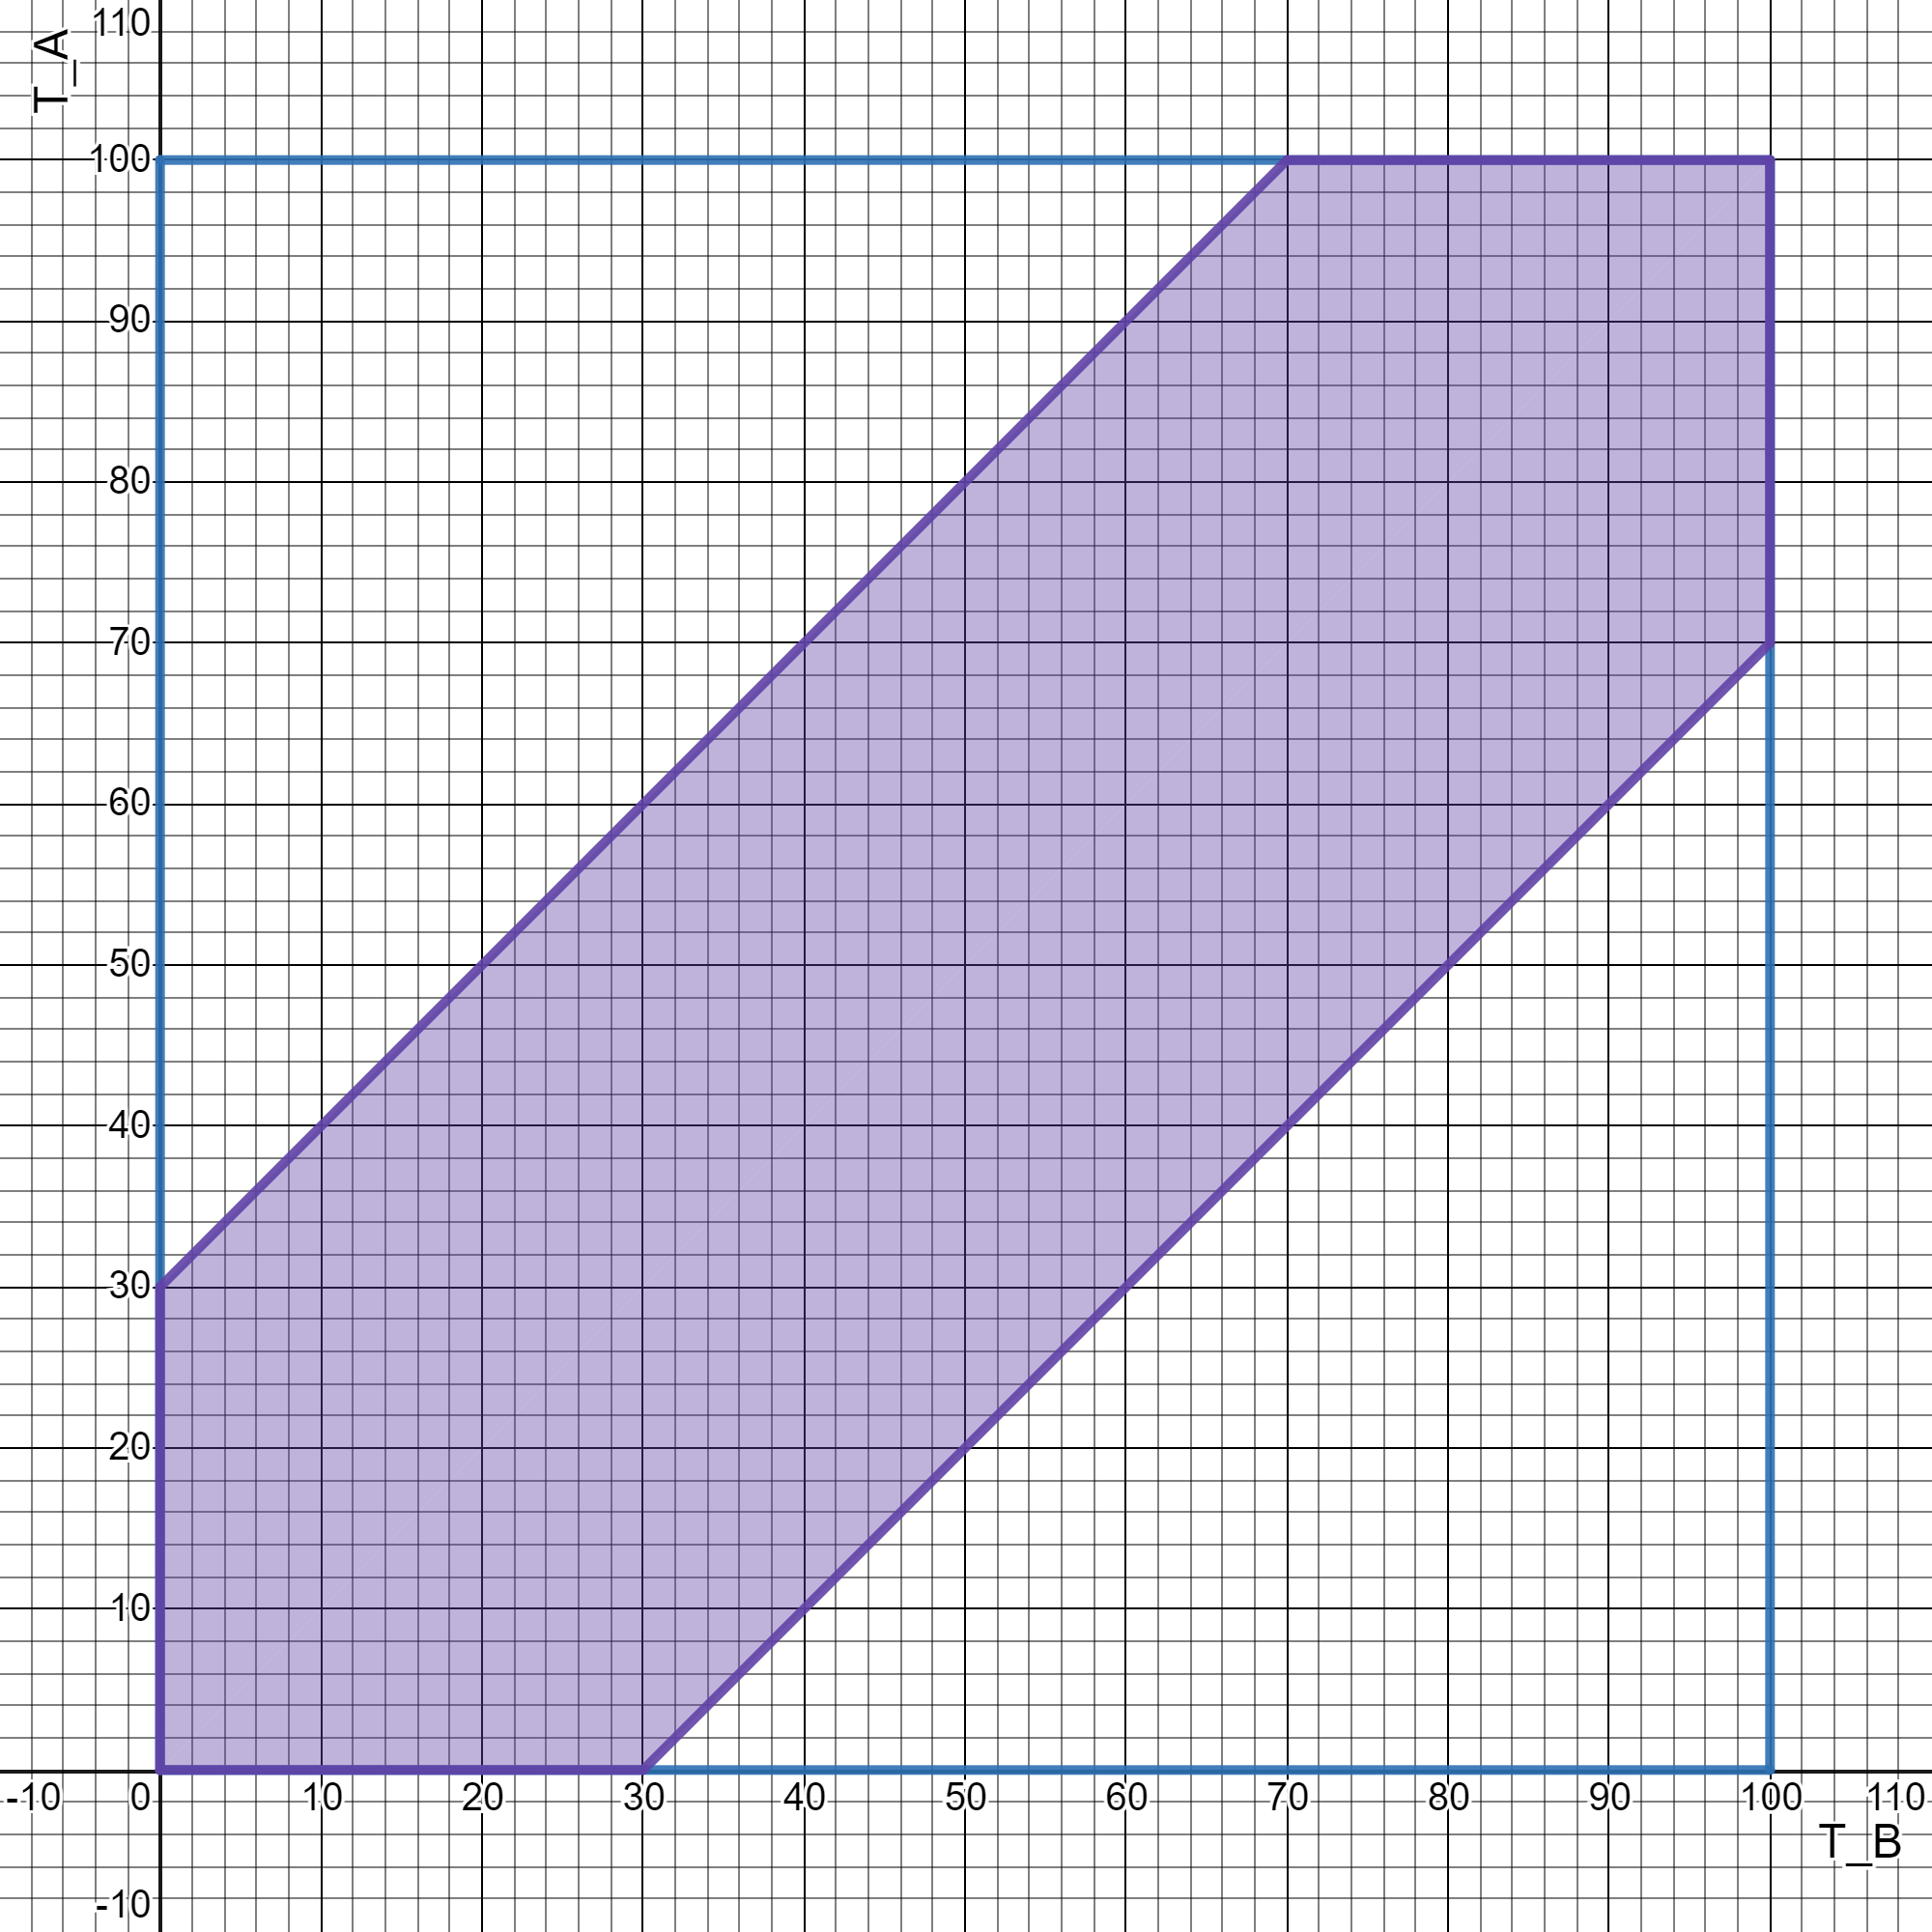
\includegraphics[width=.5\textwidth]{img/q2-d.png}
  \caption{}
\end{figure}

\begin{multicols}{2}
  \begin{itemize}
    \item $\textnormal{The area of purple part} = 5100$
    \item $\textnormal{The area of the whole part} = 10^4$
  \end{itemize}
\end{multicols}

So, the ratio of the purple area to whole area is the answer and it is $\dfrac{51}{100} = 0.51$.


\newpage
\noindent The source code (\texttt{hw4.m}) that is used for simulation.
\begin{myminted}
N = 4145; % size of Monte Carlo Simulation
total_weight = zeros(N,1); % vector to keep the total weight of vehicles for each monte carlo run

for k=1:N
    weight = 0; % the total weight for this monte carlo run

    % automobiles
    lambda = 50;      % parameter
    U = rand;         % generated uniform variable
    i = 0;            % initial value
    F = exp(-lambda); % initial value of F(0)
    while (U>=F)
        i = i + 1;
        F = F + exp(-lambda) * lambda^i / gamma(i+1);
    end

    n_a = i;        % total number of automobiles
    for j=1:n_a     % summing total weight of automobiles
        X = sum(-1/0.15 * log(rand(190,1))); % formula from example 5.11
        weight = weight + X;
    end

    % trucks
    lambda = 10;      % parameter
    U = rand;         % generated uniform variable
    i = 0;            % initial value
    F = exp(-lambda); % initial value of F(0)
    while (U>=F)
        i = i + 1;
        F = F + exp(-lambda) * lambda^i / gamma(i+1);
    end

    n_t = i;        % total number of trucks
    for j=1:n_t     % summing total weight of trucks
        X = sum(-1/0.01 * log(rand(110,1))); % formula from example 5.11
        weight = weight + X;
    end

    total_weight(k) = weight;
end

prob_over_200 = mean(total_weight > 200000);
expected_total_weight = mean(total_weight);
std_weight = std(total_weight);

fprintf('Estimated probability = %f\n', prob_over_200);
fprintf('Expected weight = %f\n', expected_total_weight);
fprintf('Standard deviation = %f\n', std_weight);

\end{myminted}


\end{document}
